\documentclass[11pt]{article}

\usepackage{microtype}
\usepackage{parskip}

\usepackage{amsmath, amssymb, amsthm}
\usepackage{mathtools, thmtools}

\usepackage[T1]{fontenc}
\usepackage[ascii]{inputenc}

\usepackage[margin=60pt]{geometry}

\usepackage{fancyhdr}
\usepackage{lastpage}

\usepackage{framed}

\usepackage{bm}

\fancypagestyle{notes}{
    \fancyhf{}
    \rhead{Monday, 11 September 2017 \\}
    \chead{\thepage\ / \pageref{LastPage} \\}
    \lhead{Math 60: Multivariable Calculus \\ Vector fields}
    %\rhead{4 September 2017}
}

\newcommand{\uvec}[1]{\bm{\hat{#1}}}
\renewcommand{\vec}[1]{\bm{#1}}

\usepackage{tikz}
\usepackage{tikz-3dplot}
\usetikzlibrary{calc, intersections}

\pagestyle{notes}

\tdplotsetmaincoords{60}{120}

\newcommand{\real}{\mathbb R}
\newcommand{\diff}{\mathrm d}

\begin{document}

\section*{What is a vector field?}

A vector field is a ``many-to-many'' function (that is, \(\mathbb R^n \to \mathbb R^m\), where \(n, m > 1\)).

\paragraph{Example}

Consider, for example, some
\[
    \vec F(x, y) = y \uvec i - x \uvec j = (y, -x).
\]
This function maps a plane to a plane (\(\real^2 \to \real^2\)), \emph{eating} two values and \emph{spitting out} two values.

To draw such a function, we might make a table:
\[
    \begin{array}{c|c}
        (x, y) & \vec F(x, y) \\ \hline
        (0, 0) & (0, 0) \\
        (1, 0) & (0, -1) \\
        (0, 1) & (1, 0) \\
        (-1, 0) & (0, 1) \\
        (0, -1) & (-1, 0) \\
    \end{array}
\]

A couple observations:
\begin{itemize}
\item The output \(\vec F(x, y)\) is always perpendicular to the input \((x, y)\), since \((x, y) \perp (y, -x) = \vec F(x, y)\).
\end{itemize}

Then, the ``graph'' of the vector field can be drawn as
\begin{center}
    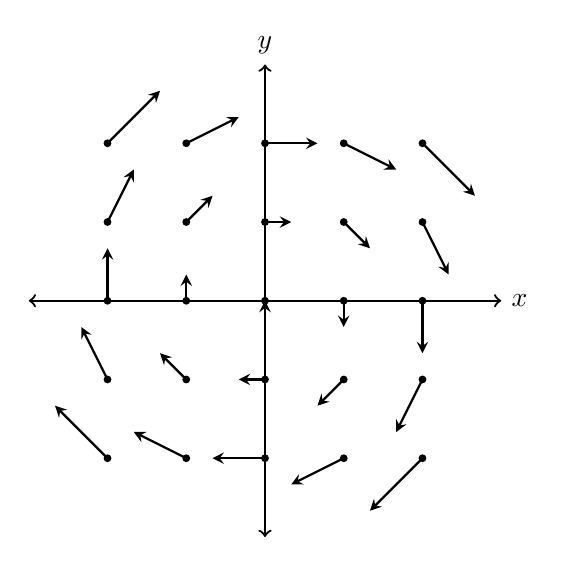
\begin{tikzpicture}
        \draw[thick, <->] 
    (-3,0) -- (3,0)
    node[right]{\(x\)};

\draw[thick, <->] 
    (0,-3) -- (0,3)
    node[above]{\(y\)};

\foreach \i in {-2,...,2} {
    \foreach \j in {-2,...,2} {
        \path
            (\i,\j) coordinate[circle, fill=black, inner sep=1pt];

        \draw[thick, ->, >=stealth]
            (\i,\j) -- ++(\j/3,-\i/3);
    }
}

    \end{tikzpicture}
\end{center}

\paragraph{Question (a very important one, most certain to appear on your test or quiz or whatever}

What are the flow lines of a given vector field \(\vec F\)?

To visualize this concept, imagine ``following'' the vector field to find a curve that traces out a ``path'' along the vector field \(\vec F\). Picture a curve \emph{tangent to} the vector field \(\vec F\) everywhere along the curve.

Then the parametrized curve \(\vec C(t) = (x(t), y(t))\) would have derivative equal to the vector field:
\[
    \diff_t \vec C (t) = \vec F(\vec C(t)).
\]

Consider the above example \(\vec F(x, y) = (y, -x)\). Then the derivative of the flow curve
\[
    \vec C'(t) = (x'(t), y'(t)) = \vec F (\vec C(t)) = (y(t), -x(t)),
\]
so that
\begin{align*}
    x'(t) &= y(t) \\
    y'(t) &= -x(t),
\end{align*}
and thus the problem is reduced to that of solving an ordinary differential equation, perhaps with some initial condition (defined, for example, by some given point through which the curve passes).

How would we solve such a differential equation?

% polynomial functions are basically like
% oh, you hit it
% oh, ow, ah, I give up
% there's another function that's very strong, that you hit it many times and it never gives up
% some function you take the derivative right, oohhh I hit I hit again 
% e^x no matter how many time you take the derivative it is still e to the x
% the log function if you take derivative ohh, 1/x it's very weak it dying
% oh, that's log log is very weak
% sin x is like a snake
% you take the derivative sin x uh huh, i'm a cosine x
% you take a derivative again and then you back to it
% this is a snake you hit it heheh, grooo, heheh, grooo~

Then, say, we might try
\begin{align*}
    x(t) &= \sin t, \\
    y(t) &= x'(t) = \cos t,
\end{align*}
and
\begin{align*}
    x(t) &= -\cos t, \\
    y(t) &= x'(t) = \sin t.
\end{align*}

Then, citing a theorem from differential equations, the general solution to this set of differential equations is given by some linear combination of the two solutions, since the two solutions are \emph{linearly independent}, since they are orthogonal: \((\sin t, \cos t) \perp (-\cos t, \sin t)\).
 
\paragraph{Velocity, speed, and acceleration}

The ``time'' derivative of some ``time-parametrized'' curve \(\vec C(t) = (x_1(t), \dots, x_n(t))\) is called the \emph{velocity vector}:
\[
    \mathbf{velocity}(t) = C'(t) = \diff_t \vec C(t) = (C_1'(t), \dots, C_n'(t)).
\]

The \emph{acceleration vector} is the second time-derivative of the curve:
\[
    \mathbf{acceleration}(t) = \vec C''(t) = \diff_t^2 \vec C(t) = (C_1''(t), \dots, C_n''(t)).
\]

The \emph{speed}, or the absolute value (``magnitude'') of the velocity, is geometrically the length of the velocity vector:
\[
    \mathrm{speed}(t) = |\mathbf{velocity}(t)| = \sqrt{(C_1'(t))^2 + \dots + (C_n'(t))^2}.
\]

\paragraph{Example}

Take some parametrized curve \(\vec C(t) = (\cos t, \sin t, t)\). Then the velocity vector is
\[
    \vec C'(t) = (-\sin t, \cos t, 1),
\]
the speed is
\[
    |\vec C'(t)| = \sqrt{(-\sin t)^2 + (\cos t)^2 + (1)^2} = \sqrt{2},
\]
and the acceleration is
\[
    \vec C''(t) = (-\cos t, -\sin t, 0).
\]

Some terms: a curve with speed \(1\) is said to have \emph{unit speed}, and curves that run in \emph{unit speed} are said to be \emph{parametrized by arclength}.

\paragraph{Distinctions between the ``image'' and the function}

Consider some possible parametrization of a circle
\begin{align*}
    \vec \alpha(t) &= (\cos t, \sin t), \quad 0 \le t < 2\pi, \\
    \vec \beta(t) &= (\sin t, \cos t), \quad 0 \le t < 2\pi, \\
    \vec \gamma(t) &= (\cos 2\pi t, \sin 2 \pi t), \quad 0 \le t < 1.
\end{align*}
The ``path'' of the curves look something like
\begin{center}
    
\end{center}
Notice that these curves have different starting points and/or different orientations (directions) and/or different speeds. Consequently, even though the images traced out by the curves are the same, the curves themselves are \emph{not} the same.

\paragraph{Arc length}

The arc length is given by the integral of speed over time:
\[
    S = \int_t |\vec C'(t)| \, \diff t.
\]




\end{document}



